\chapter{DESARROLLO DEL EXPERIMENTO}
\section{Construcción de los conjuntos finales de datos}

\section{Análisis Exploratorios de los datos}
De los 27,251 proyectos tecnológicos obtenidos de Kickstarter, la distribución según el estado de financiamiento va según la Figura \ref{4:fig1}.
\begin{figure}[h]
	\begin{center}
		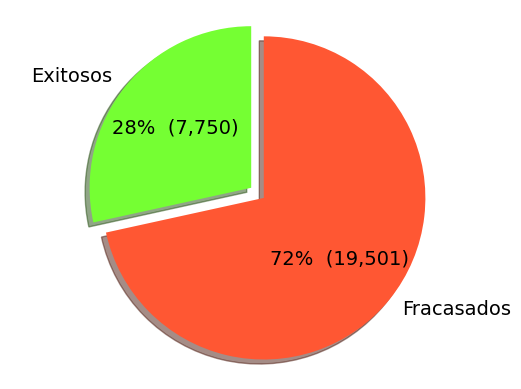
\includegraphics[width=0.7\textwidth]{4/figures/projects by state.png}
		\caption{Distribución total de proyectos tecnológicos por su estado. Fuente: Elaboración propia.}
		\label{4:fig1}
	\end{center}
\end{figure}


Asimismo, la Figura \ref{4:fig2} muestra la distribución de los estos proyectos por año, desde el 2009 hasta el 2019.

\begin{figure}[h]
	\begin{center}
		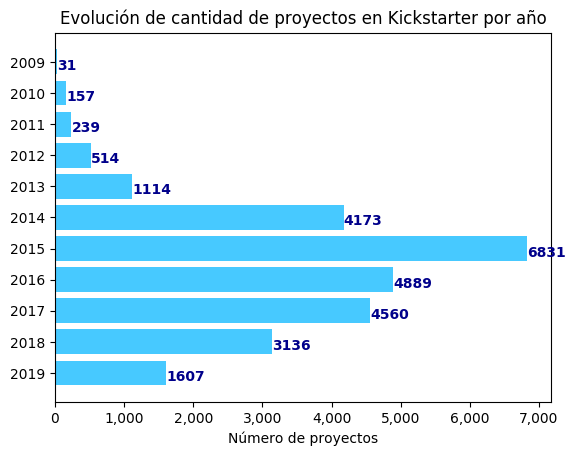
\includegraphics[width=0.8\textwidth]{4/figures/projects state by year.png}
		\caption{Evolución de cantidad de proyectos tecnológicos por año. Fuente: Elaboración propia.}
		\label{4:fig2}
	\end{center}
\end{figure}


La misma evolución pero detallada por el estado de financiamiento se observa en la Figura \ref{4:fig3}.

\begin{figure}[h]
	\begin{center}
		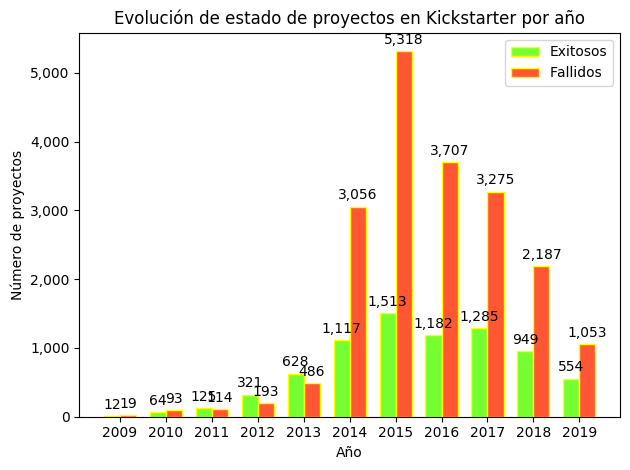
\includegraphics[width=0.8\textwidth]{4/figures/projects state evolution by year.png}
		\caption{Evolución de proyectos tecnológicos, por su estado y año. Fuente: Elaboración propia.}
		\label{4:fig3}
	\end{center}
\end{figure}

\subsection{Metainformación}

\subsection{Descripciones}

\subsection{Comentarios}
Al analizar los proyectos exitosos y fracasados de acuerdo a la presencia de comentarios (Figura \ref{4:fig4}), se observa que hay una sólida relación entre aquellos que fracasaron y los que no cuentan con comentarios, mientras que para los proyectos exitosos, la asociación es menos contundente ya que la diferencia entre aquellos que presentan comentarios y los que no es menor.

\begin{figure}[h]
	\begin{center}
		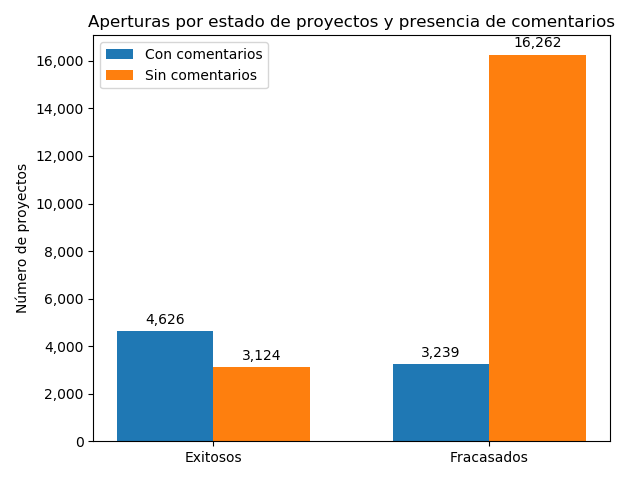
\includegraphics[width=0.8\textwidth]{4/figures/projects state by comment.png}
		\caption{Aperturas de proyectos por estado de financiamiento y presencia de comentarios. Fuente: Elaboración propia.}
		\label{4:fig4}
	\end{center}
\end{figure}

Si se repite el ejercicio del análisis anterior, ahora partiendo de los comentarios por presencia de comentarios y abiertos por su estado de financiamiento (exitosos y fracasados), se visualiza en la Figura \ref{4:fig5} una relación casi idéntica al anterior gráfico de barras.

\begin{figure}[h]
	\begin{center}
		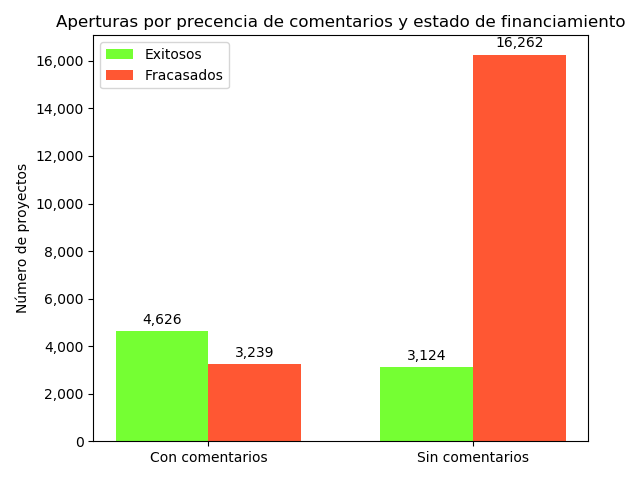
\includegraphics[width=0.8\textwidth]{4/figures/projects comment by state.png}
		\caption{Aperturas de proyectos por presencia de comentarios y estado de financiamiento. Fuente: Elaboración propia.}
		\label{4:fig5}
	\end{center}
\end{figure}

Por último, del universo de proyectos tecnológicos que presentan comentarios, los más de 4 mil proyectos exitosos contienen casi la totalidad de comentarios registrados (97\%), representando más de 475 mil como se aprecia en la Figura \ref{4:fig6}. Estos datos confirma la correlación existe entre la presencia de un volumen considerable de comentarios y su éxito de financiación.

\begin{figure}[h]
	\begin{center}
		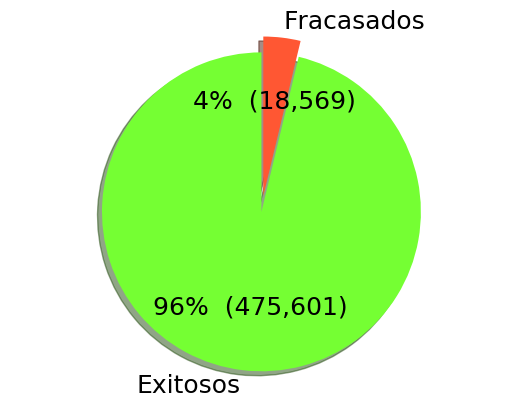
\includegraphics[width=0.8\textwidth]{4/figures/total comments by projects state.png}
		\caption{Distribución de comentarios en proyectos exitosos y fracasados. Fuente: Elaboración propia.}
		\label{4:fig6}
	\end{center}
\end{figure}

\section{Pre-procesamiento de los conjuntos de datos}

\section{Creación de los modelos predictivos}
